\chapter{\label{ch:dev}Development practices}

As this is a new software project, we invested a significant effort in setting
up a development infrastructure to ensure our work is tracked,
thoroughly and continually tested, and incrementally improved and documented.
To this end, we have adopted best practices for software development used by
successful open source projects \cite{millman2014}.

\section{\label{sec:vc}Version control}

We use Git\footnote{\url{http://git-scm.com}} as our version control system
(VCS) and GitHub\footnote{\url{https://github.com}} as the public hosting
service for our official \texttt{upstream} repository
\url{https://github.com/statlab/permute}.  Git allows us to track and manage
how our code changes over time as well as review all new functionality before
merging it into the main codebase.  To get new code integrated in the official
\texttt{upstream} repository, we use GitHub's \emph{pull request} mechanism.
This enables us to review code before integrating it.  In the following
section, I describe how we automate our testing to generate reports for all
pull request.  This way we can verify that changes to our code don't break
existing functionality.  Once a pull request is reviewed and accepted, it is
then --- and only then --- merged into the \texttt{upstream} repository.

%To summarize, all new work is made on a branch and pushed to our
%personal forks of the upstream repository. To incorporate this new
%work on our local master branch we then pull from the upstream
%master.  This separation between where we push and pull our
%work creates the space for code review, testing, and discussion of
%new features and bugfixes before merging work into the official 
%repository.

\section{\label{sec:test}Testing}

We use the \texttt{nose} testing framework for automating our testing
procedures.\footnote{\url{https://nose.readthedocs.org}}  This is the standard
testing framework used by the core packages in the scientific Python ecosystem.
Automating the tests allows us to monitor a proxy for code correctness when
making changes as well as simplifying the code review process for new code. 
The \texttt{nose} testing framework simplifies test creation, discovery,
and running. It has an extensive set of plugins to add functionality
for coverage reporting, test annotation, profiling, isolation, as well
as inspecting and testing documentation.

%we've primarily used it for testing individual units of code for
%consistency.  Eventually we will add regression and integration testing as well
%as testing the code for correctness using the expected statistical properties.
%For instance, rather than merely checking whether when a function is called
%with the same arguments it returns the same results, we can run tests that
%check whether results are within the expected statistical error.
%
%While testing is not a proof of program correctness, it can serve as a
%useful tool for catching errors and increase our confidence in the
%reliability of our results.

%For example, from the top-level of the repository, you can ask \texttt{nose}
%to run the tests by entering \texttt{nosetests permute} in Bash.  For example,
%
%\begin{verbatim}
%$ nosetests permute
%.......................................
%----------------------------------------------------------------------
%Ran 39 tests in 48.957s
%\end{verbatim}
%
%In the above console output, you will see a ``.'' for each test, which
%is run.  A test corresponds to a function and each test may test several
%things.

%\subsection{Coverage}

%We also use \texttt{nose} to monitor our test coverage.  

\begin{figure}
  \begin{centering}
    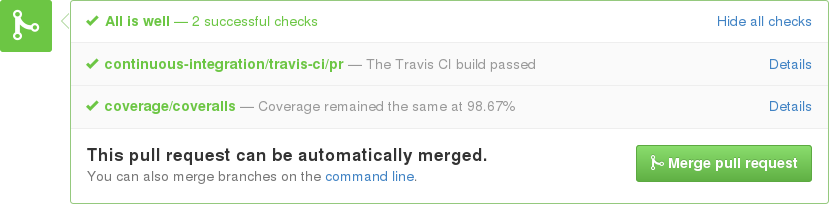
\includegraphics[width=\textwidth]{fig/pull-request-ci.png}\par
  \end{centering}

  \caption{\label{fig:pull-request}Pull request and continuous integration.}
\end{figure}

Our goal is to test every line of code.  For example, not only do we want to
test every function in our package, but if a specific function has internal
logic we want to test each possible path through the function.  Having tested
each line of code increases our confidence in our codebase, but more
importantly provides us assurance that changes we make do not break existing
code.  It also increases our confidence that new code works, which reduces the
friction of accepting contributions.  Currently over 98\% of our code has at
least one test touch it.

%Working in the top-level of our local repository in Bash, you could
%enter
%
%\begin{verbatim}
%$ nosetests permute --with-coverage --cover-package=permute
%.......................................
%Name                 Stmts   Miss Branch BrMiss  Cover   Missing
%----------------------------------------------------------------
%permute                 43      5     10      1    89%   77-88
%permute.core            60      0     30      4    96%   
%permute.data            45      0      2      0   100%   
%permute.eda             22      0      8      0   100%   
%permute.irr             52      0     20      1    99%   
%permute.stratified      45      0     16      1    98%   
%permute.utils           10      0      6      0   100%   
%----------------------------------------------------------------
%TOTAL                  277      5     92      7    97%   
%----------------------------------------------------------------------
%Ran 39 tests in 56.023s
%
%OK
%\end{verbatim}
%Here you can see, that in addition to running 39 tests without error,


%The remaining
%lines are mostly branch misses where executing both branches is difficult.  For
%example, the branch depends on the particular environment in which it is being
%run. So each branch is tested in different environments, but not at the same
%time.  I've tried to trick the tests to run both branches by hand modifying
%system objects in the tests as well as creating mock objects, but haven't been
%able to achieve 100\% coverage.

%\subsection{Continuous integration}

%Having an automated test suite enables us to implement continuous integration.
%Continuous integration is the process of automatically running the full test
%suite i

We've configured Travis CI\footnote{\url{https://travis-ci.org}} and
\texttt{coveralls}\footnote{\url{https://coveralls.io}} to be automatically
triggered whenever a commit is made to a pull request or the upstream
master directly.  These systems then run the full test suite 
using different versions of our dependencies (e.g., Python 2.7 and 3.4) %on
%different operating systems (e.g., Windows, Mac OS, and Linux) 
every time a
new commit is made to a repository or pull request.
This means that when you go to review a pull request you can immediately see
a full report of whether the change breaks any of the tests as well as whether
the new code decreases the overall test coverage.

%Python 2 and Python 3 on Debian-derived system
%
%I run the tests for both Python 2 and Python 3 on a RedHat-derived system
%
%While Philip and Kellie run the tests for Python 2 on Mac OS.
%
%need to add additional build systems to buildbot nipy.bic.berkeley.edu...
%
%\texttt{coveralls}\footnote{\url{https://coveralls.io}}
%

\section{\label{sec:doc}Documentation}

%Reducing the friction involved with producing documentation encourages
%developers and users to contribute documentation.  For instance, NumPy use to
%have fairly poor documentation until one summer when Stefan van der Walt (now a
%BIDS fellow) built on several newly improved Python technologies for
%documentation \cite{SciPyProceedings_27}.

We use Sphinx\footnote{\url{http://sphinx-doc.org}} as our documentation system
and already have good developer documentation and the foundation for
high-quality user documentation. We've used Python docstrings and the NumPy
docstring standard to document all the modules and functions in
\texttt{permute}.\footnote{\url{https://github.com/numpy/numpy/blob/master/doc/HOWTO\_DOCUMENT.rst.txt}}
Using Sphinx and some NumPy extensions, we have a system for autogenerating the
project documentation (as HTML or PDF) using the docstrings as well as
stand-alone text written in a light-weight markdown-like language.  This
enables us to embed references, figures, code that is auto-run during
documentation generation, as well as mathematics using \LaTeX.

%- ``cite McNell et al. as soon as we introduce the gender bias example in the notebook.''
%
%\cite{macnell2014s}

\section{\label{sec:release}Release management}

Our development workflow ensures that the official \texttt{upstream} repository
is always pristine and ready for use.  This means anyone can get our official
upstream master at any point, install it and start using it.  We also 
make official releases with ``binary'' packages\footnote{Presently our code is pure
Python, but we release Python wheels.}
uploaded to the Python Package Index, or PyPI, with release announcements posted
to our mailing list.
To install the latest release of \texttt{permute} and its dependencies, type
the following command from a Bash prompt (assuming you have Python and a recent version of pip): 

\texttt{\$ pip install permute}
%This will install version 0.1.alpha0 of \texttt{permute} as well as it
%dependencies.  Since we have yet to finalize our call signatures or package
%structure, we use the alpha designation to telegraph this fact to
%potential users.  However, our release process is fully documented and
%partially automated.  Together with the policy of keeping upstream master
%pristine, this means that making new releases is extremely light-weight.  Being
%able to quickly generate new releases quickly and reliably is essential to being able to
%quickly respond to mistakenly broken releases.  Despite using a rigorous
%testing and integration methodology, error is a constant concern.  Being able
%to quickly respond to discovered errors in released software is essential to
%creating a software tool people trust.
